\section{Optimizations}
\label{SECTION_Optimizations}

\subsection{Random Forests}
\label{SUBSECTION_RandomForests}

The developed decision tree classifier within the Baseline didn’t turn out to be a good choice in terms of achieving the best accuracy. So, using Ensemble techniques, we’ll be using this section to explain the training process of a Random Forest Classifier, as well as the hyperparameter tuning process we’ve performed\footnote{Refer to: \texttt{Task02\_SupervisedLearning\_RandomForests\_Barba\_Guerrero\_Schmidt.ipynb}.}.

As a starting point, we ran the \texttt{RandomForestClassifier} model provided by sklearn without any complex parameters to create a baseline F1 score. The only parameter we use is the amount of estimators \texttt{n\_estimators} determining the amount of Decision Trees in our Random Forest. Using 100, we achieve a score of 0.7020, which is interesting, considering that our manually tuned decision trees achieved a score 0.77\% worse.

Generally, comparing Random Forests to Decision Trees, there are even more parameters which are also even less intuitive to understand. For instance, instead of five parameters for the final classifier, we use eight. These, adding to the problem, each interact with each other. This makes choosing the right combination of parameters quite difficult. The problem of choosing the combination yielding the most accurate results can be found using specialized search tools. Within the project, we used both Randomized Search, and Grid Search.

Randomized search is a technique where a range of hyperparameter values is defined, and a random sample of these values is selected and used to train and evaluate the model. This technique is not exhaustive and was used to gain a general idea of the ideal hyperparameter ranges. In multiple cycles, we modified a list of parameters to test, and evaluated the outcomes. 

After about four to five hours of code executions, we compiled a list of insights during four testing cycles. Figure \ref{PICTURE_figure_rf_01} shows the final values within cycle 3 and 4.

\begin{figure}[h!]
	\centering
            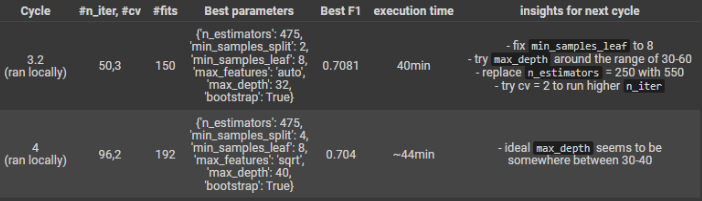
\includegraphics[width=120mm]{images/rf_figure_01.png}
	\caption{Iterative insights during Random Forest Hyperparameter Tuning.}
	\label{PICTURE_figure_rf_01}
\end{figure}

Up until now, the best F1 score we could achieve is 0.7081 (0.7123 as evaluated on DrivenData.org) suggesting that there might not be as much potential to this technique as we initially hoped for. 

In order to find the final set of hyperparameters, we use the Grid Search technique. Grid search is a technique where a grid of hyperparameter values is defined, and the model is trained and evaluated using all possible combinations of these values. This can be an exhaustive and time-consuming process, but it is effective for finding the optimal hyperparameter values for a model. The outcome values of the Randomized Search and those very close to them are chosen for the grid of possible parameters. By doing this, we unfortunately weren’t able to improve our F1 score in comparison to the Randomized Search approach and yielded a score of 0.704.

Taking a look at the improvements related to Decision Trees and its Ensemble version, the Random Forest, we see that this type of classifier is not suited enough for the classification task at hand - Other classifiers developed in this project had achieved a score greater than 0.74. Figure \ref{PICTURE_figure_rf_02} shows all results side-by-side, including a comparison to the best result of the competition at the time of writing, the 12th of December 2022.

\begin{figure}[h!]
	\centering
            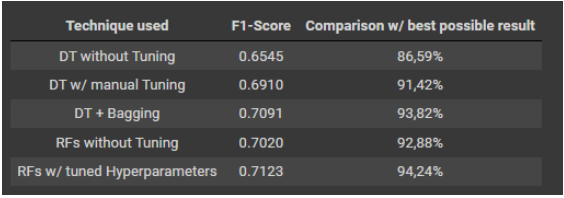
\includegraphics[width=80mm]{images/rf_figure_02.png}
	\caption{Random Forest: Achieved improvements from Hyperparameter Tuning.}
	\label{PICTURE_figure_rf_02}
\end{figure}


\subsection{XGBoost}
\label{SUBSECTION_XGBoost}
After developing a proper baseline model that gave us results of up to 0.7215 accuracy, the next idea is to start implementing more and more complex models to try to reach the top spots. Using XGBoost, a priori, we expect better results (with the same features obtained from the decision trees), as it is known for being a better model that could be good when trying to make these kinds of predictions that we are trying to do. Historically, it has been good to make predictions in this competition, so we try to use it to improve our results in it \footnote{Refer to: \texttt{Task02\_SupervisedLearning\_XGBoost\_Barba\_Guerrero\_Schmidt.ipynb}.}.

Using the base model without further hyperparameter tuning, we get a f1-score of 0.7183, which seems pretty good at first. Regarding hyperparameter tuning, it can be done in these ways:
\begin{enumerate}
    \item We will perform random search to obtain possible good values for the hyperparameters.
    \item We will perform grid search to obtain the "optimal" values for the hyperparameters.
\end{enumerate}

Using the first option, we can get rank 695, as we got a result of 0.7364. On the other hand, the second option gets us to rank 668, with a score of 0.7378. However, we still believe that it can be improved, either by normalizing the data or using Bayes search. Unfortunately, none of these seem to produce better models, most likely because it did not finish the execution (it did not converge) in the latter case.

In this section, AdaBoost and GradientBoost were also tested, but failed to show improvements versus the previous models.
\subsection{CatBoost}
\label{SUBSECTION_CatBoost}

After the previous tests, CatBoost was used, in order to look for a better model than the previously mentioned \footnote{Refer to: \texttt{Task02\_SupervisedLearning\_CatBoost\_Barba\_Guerrero\_Schmidt.ipynb}.}. The idea in this section is to take advantage of CatBoost virtue to work with categorical variables and apply it to the 3 geo level columns.

Since it requires very little parametrization, it is quite easy and fast to implement, providing a noticeably high f1-score.

\subsection{LightGBM}
\label{SECTION_LightBGM}

Another good strategy to improve the model accuracy is to use LightGBM for gradient boosting as well\footnote{Refer to: \texttt{Task02\_SupervisedLearning\_LightGBM\_Barba\_Guerrero\_Schmidt.ipynb}.}. For the cross validation, we used 5 folds of 100 candidates each, equalling 500 fits in total.

This model, along a proper parametrization, also seems promising at first, so we will include it in other complex models.

The link to the Google Colab document for LightGBM is the following:

\subsection{Basic Stacked Model}
\label{SUBSECTION_BSM}

Having considered all the previous models, we can dedicate ourselves in this section to construct a stacked model containing several of the previously developed ones\footnote{Refer to: \texttt{Task02\_SupervisedLearning\_BasicStackedModel\_Barba\_Guerrero\_Schmidt.ipynb}.}.

In our case, the model providing the best results consists in the combination of the XGBoost one, the baseline KNN model and the baseline DT model. All values here are normalized for improved performance after testing the not normalized ones.

Regarding the stacked model, we will use stratified K-fold cross validation with 5 splits, and logistic regression. Testing the basic stacked model gives us a f1-score of 0.7499, representing a huge 0.7423 value in the competition, for a rank of 532. As always, this difference may be caused by a bit of overfitting in the model.

Here, one would think that including the boosted model would significantly help to achieve a better result, but it turns out it is not the case. We tried adding both the LightGBM model and the CatBoost model, only for us to get a f1-score of 0.7483, versus the previous 0.7499.